% Paquets généraux
\documentclass[a4paper,12pt,titlepage,twoside]{article}
\usepackage[utf8x]{inputenc}
\usepackage[T1]{fontenc}
\usepackage[french]{babel}
\usepackage{textgreek}
\usepackage[gen]{eurosym}
%\usepackage[dvips]{graphicx}
\usepackage{fancyhdr}
\usepackage{pdfpages}
\usepackage{multido}
\PassOptionsToPackage{obeyspaces}{url}
\usepackage{hyperref}
\usepackage{numprint}
\nplpadding{2}
\usepackage{pstricks}
%\usepackage{aeguill}
\usepackage{listings}

\newcommand{\id}{140}
\newcommand{\nom}{Découverte des sytèmes}
\newcommand{\sequence}{01}
\newcommand{\nomsequence}{Analyse fonctionnelle}
\newcommand{\num}{01}
\newcommand{\type}{TP}
\newcommand{\descrip}{TP qui consiste à découvrir les systèmes en effectuant des petites acquisitions.}
\newcommand{\competences}{D2-06: Justifier le choix d'un capteur ou d'un appareil de mesure vis-à-vis de la grandeur physique à mesur \\ &  D3-04: Identifier les erreurs de mesure. \\ &  D3-05: Identifier les erreurs de méthode.}
\newcommand{\nbcomp}{3}
\newcommand{\systemes}{Moteur à courant continu}
\newcommand{\systemesnum}{86}
\newcommand{\systemessansaccent}{Moteur a courant continu}
\newcommand{\ilot}{1}
\newcommand{\ilotstr}{01}
\newcommand{\dossierilot}{\detokenize{Ilot_01 Moteur à courant continu}}
\newcommand{\imageun}{Moteur_a_courant_continu}


\newcommand\twodigits[1]{%
   \ifnum#1<10 0#1\else #1\fi
}

\newcommand{\auteurun}{Renaud Costadoat}
\newcommand{\auteurdeux}{Françoise Puig}
\newcommand{\auteurs}{Costadoat - Puig}
\newcommand{\institute}{Lycée Dorian}
\newcommand{\competensequestion}{}
\usepackage{color}
\usepackage{xcolor}
\usepackage{colortbl}
\usepackage{helvet}
\usepackage[frenchmath]{newtxsf} % for sans serif symbols
\renewcommand{\familydefault}{\sfdefault}
%\usepackage{amsfonts}
%\usepackage{amsmath}
%\usepackage{lmodern}
\usepackage{mathastext}
%\usepackage{xspace}
\usepackage{varioref}
\usepackage{tabularx}
%\usepackage{floatflt}
\usepackage{graphics}
\usepackage{wrapfig}
\usepackage{textcomp}
\usepackage{tikz}
\usepackage{wrapfig}
\usepackage{gensymb}
\usepackage[european]{circuitikz}
\usetikzlibrary{babel}
\usetikzlibrary{arrows}
\usetikzlibrary{positioning}
\usepackage{ifthen}
\usepackage{cancel}
\usepackage{etoolbox}
\usepackage{multirow}
%\usepackage{boxedminipage}
\definecolor{gris25}{gray}{0.75}
\definecolor{analyser}{RGB}{196,189,151}
\definecolor{analyserf}{RGB}{73,69,41}
\definecolor{modeliser}{RGB}{252,213,180}
\definecolor{modeliserf}{RGB}{226,107,10}
\definecolor{resoudre}{RGB}{216,228,188}
\definecolor{resoudref}{RGB}{118,147,60}
\definecolor{experimenter}{RGB}{230,184,183}
\definecolor{experimenterf}{RGB}{150,54,52}
\definecolor{concevoir}{RGB}{141,180,226}
\definecolor{concevoirf}{RGB}{15,36,62}
\definecolor{realiser}{RGB}{184,204,228}
\definecolor{realiserf}{RGB}{54,96,146}
\definecolor{communiquer}{RGB}{204,192,218}
\definecolor{communiquerf}{RGB}{96,73,122}
\definecolor{bleu}{RGB}{18,33,98}
\definecolor{bleutf}{RGB}{8,53,154}
\definecolor{bleuf}{RGB}{42,94,171}
\definecolor{bleuc}{RGB}{159,194,225}
\definecolor{rougef}{RGB}{185,18,27}
\definecolor{rougec}{RGB}{255,188,204}%255,230,231
\definecolor{vertf}{RGB}{103,126,82}
\definecolor{vertc}{RGB}{220,255,191}
\definecolor{forestgreen}{rgb}{0.13,0.54,0.13}
\definecolor{blcr}{rgb}{0.59,0.69,0.84}
\definecolor{blfr}{rgb}{0.32,0.51,0.75}
\definecolor{orfr}{RGB}{251,86,35}
\definecolor{orcr}{rgb}{0.90,0.65,0.50}
\definecolor{orangef}{rgb}{0.89,0.56,0.16}
\definecolor{orange}{rgb}{0.58,0.35,0.063}
\definecolor{orangec}{rgb}{0.94,0.76,0.56}
\definecolor{rcorrect}{rgb}{0.6,0,0}
\definecolor{sequence}{rgb}{0.75,0.75,0.75}
\definecolor{competences}{rgb}{0.61,0.73,0.35}
\definecolor{grisf}{HTML}{222222}
\definecolor{grisc}{HTML}{636363}
\definecolor{normal}{HTML}{4087c4}
\definecolor{info}{HTML}{5bc0de}
\definecolor{success}{RGB}{92,184,92}
\definecolor{warning}{RGB}{240,173,78}
\definecolor{danger}{RGB}{217,83,79}
\definecolor{darkWhite}{rgb}{0.94,0.94,0.94}

\hypersetup{                    % parametrage des hyperliens
    colorlinks=true,                % colorise les liens
    breaklinks=true,                % permet les retours à la ligne pour les liens trop longs
    urlcolor= blfr,                 % couleur des hyperliens
    linkcolor= orange,                % couleur des liens internes aux documents (index, figures, tableaux, equations,...)
    citecolor= forestgreen                % couleur des liens vers les references bibliographiques
    }


\lstset{
  aboveskip=3mm,
  belowskip=-2mm,
  backgroundcolor=\color{darkWhite},
  basicstyle=\footnotesize,
  breakatwhitespace=false,
  breaklines=true,
  captionpos=b,
  commentstyle=\color{red},
  deletekeywords={...},
  escapeinside={\%*}{*)},
  extendedchars=true,
  framexleftmargin=16pt,
  framextopmargin=3pt,
  framexbottommargin=6pt,
  frame=tb,
  keepspaces=true,
  keywordstyle=\color{blue},
  language=C,
  literate=
  {²}{{\textsuperscript{2}}}1
  {⁴}{{\textsuperscript{4}}}1
  {⁶}{{\textsuperscript{6}}}1
  {⁸}{{\textsuperscript{8}}}1
  {€}{{\euro{}}}1
  {é}{{\'e}}1
  {è}{{\`{e}}}1
  {ê}{{\^{e}}}1
  {ë}{{\¨{e}}}1
  {É}{{\'{E}}}1
  {Ê}{{\^{E}}}1
  {û}{{\^{u}}}1
  {ù}{{\`{u}}}1
  {â}{{\^{a}}}1
  {à}{{\`{a}}}1
  {á}{{\'{a}}}1
  {ã}{{\~{a}}}1
  {Á}{{\'{A}}}1
  {Â}{{\^{A}}}1
  {Ã}{{\~{A}}}1
  {ç}{{\c{c}}}1
  {Ç}{{\c{C}}}1
  {õ}{{\~{o}}}1
  {ó}{{\'{o}}}1
  {ô}{{\^{o}}}1
  {Õ}{{\~{O}}}1
  {Ó}{{\'{O}}}1
  {Ô}{{\^{O}}}1
  {î}{{\^{i}}}1
  {Î}{{\^{I}}}1
  {í}{{\'{i}}}1
  {Í}{{\~{Í}}}1,
  morekeywords={*,...},
  numbers=left,
  numbersep=10pt,
  numberstyle=\tiny\color{black},
  rulecolor=\color{black},
  showspaces=false,
  showstringspaces=false,
  showtabs=false,
  stepnumber=1,
  stringstyle=\color{gray},
  tabsize=4,
  title=\lstname,
}

% Mise en page
\pagestyle{fancy}

\setlength{\hoffset}{-18pt}

\setlength{\oddsidemargin}{0pt} 	% Marge gauche sur pages impaire2s
\setlength{\evensidemargin}{0pt} 	% Marge gauche sur pages paires
\setlength{\marginparwidth}{00pt} 	% Largeur de note dans la marge
\setlength{\headwidth}{481pt} 	 	% Largeur de la zone de tête (17cm)
\setlength{\textwidth}{481pt} 	 	% Largeu\textbf{r de la zone de texte (17cm)
\setlength{\voffset}{-18pt} 		% Bon pour DOS
\setlength{\marginparsep}{7pt}	 	% Séparation de la marge
\setlength{\topmargin}{-30pt} 		% Pas de marge en haut
\setlength{\headheight}{45pt} 		% Haut de page
\setlength{\headsep}{20pt} 			% Entre le haut de page et le texte
\setlength{\footskip}{30pt} 		% Bas de\textbf{ page + séparation
\setlength{\textheight}{700pt} 		% Hauteur de l'icone zone de texte (25cm)
\setlength\fboxrule{1 pt}
\renewcommand{\baselinestretch}{1}
\setcounter{tocdepth}{1}
\newcommand{\cadre}[2]
{\fbox{
  \begin{minipage}{#1\linewidth}
   \begin{center}
    #2\\
   \end{center}
  \end{minipage}
 }
}

\newcounter{num_quest} \setcounter{num_quest}{0}
\newcounter{num_rep} \setcounter{num_rep}{0}
\newcounter{num_cor} \setcounter{num_cor}{0}

\newcommand{\question}[1]{\refstepcounter{num_quest}\par
~\ \\ \parbox[t][][t]{0.15\linewidth}{\textbf{Question \arabic{num_quest}}}\parbox[t][][t]{0.85\linewidth}{#1}\par
}


\newcommand{\questioncomp}[2]{
\ifthenelse{\equal{#1}{ana}}{\renewcommand{\competensequestion}{\textcolor{analyserf}{Analyser}}}{
\ifthenelse{\equal{#1}{mod}}{\renewcommand{\competensequestion}{\textcolor{modeliserf}{Modéliser}}}{
\ifthenelse{\equal{#1}{res}}{\renewcommand{\competensequestion}{\textcolor{resoudref}{Résoudre}}}{
\ifthenelse{\equal{#1}{exp}}{\renewcommand{\competensequestion}{\textcolor{experimenterf}{Expérimenter}}}{
\ifthenelse{\equal{#1}{con}}{\renewcommand{\competensequestion}{\textcolor{concevoirf}{Concevoir}}}{
\ifthenelse{\equal{#1}{rea}}{\renewcommand{\competensequestion}{\textcolor{realiserf}{Réaliser}}}{
\ifthenelse{\equal{#1}{com}}{\renewcommand{\competensequestion}{\textcolor{communiquerf}{Communiquer}}}{
}}}}}}}
\refstepcounter{num_quest}\par
~\ \\ \parbox[t][][t]{0.18\linewidth}{\textbf{Question \arabic{num_quest}}\\ \competensequestion}\parbox[t][][t]{0.8\linewidth}{#2}\par
}

\newcommand{\urlgithub}[1]{https://raw.githubusercontent.com/Costadoat/Sciences-Ingenieur/master/}

\newcommand{\dossiergithub}[1]{\urlgithub/S\sequence\%20\nomsequence/\type\num\%20\nom/}

\newcommand{\urlsysteme}{\href{https://www.costadoat.fr/systeme/\systemesnum}{système}}

\newcommand{\reponse}[1]
{\refstepcounter{num_rep}
\noindent
\rule{\linewidth}{.5pt}
\textbf{Question \arabic{num_rep}:}
\multido{\i=1+1}{#1}{~\ \\}
}

\newcommand{\cor}
{\refstepcounter{num_cor}
\noindent
\rule{\linewidth}{.5pt}
\textbf{Question \arabic{num_cor}:} \\
}

\newcommand{\titre}[1]
{\begin{center}
\cadre{0.8}{\huge #1}
\end{center}
}

%Titres des sections

\newcommand{\titleana}[2]{%
\tikzstyle{titlebox}=[rectangle,inner sep=10pt,inner ysep=10pt,draw,fill=analyser]%
\tikzstyle{title}=[fill=analyser]%
%
\bigskip\noindent\begin{tikzpicture}
\node[titlebox] (box){%
\begin{minipage}{0.94\textwidth}
\textbf{\textcolor{analyserf}{#1}}
\end{minipage}
};
%\draw[color=blue] (box.north west)--(box.north east);
\node[title] at (box.north) {\textcolor{analyserf}{ANALYSER}};
\end{tikzpicture}%
\\}

\newcommand{\titlemod}[2]{%
\tikzstyle{titlebox}=[rectangle,inner sep=10pt,inner ysep=10pt,draw,fill=modeliser]%
\tikzstyle{title}=[fill=modeliser]%
%
\bigskip\noindent\begin{tikzpicture}
\node[titlebox] (box){%
\begin{minipage}{0.94\textwidth}
\textbf{\textcolor{modeliserf}{#1}}
\end{minipage}
};
%\draw[color=blue] (box.north west)--(box.north east);
\node[title] at (box.north) {\textcolor{modeliserf}{MODELISER}};
\end{tikzpicture}%
\\}

\newcommand{\titleres}[2]{%
\tikzstyle{titlebox}=[rectangle,inner sep=10pt,inner ysep=10pt,draw,fill=resoudre]%
\tikzstyle{title}=[fill=resoudre]%
%
\bigskip\noindent\begin{tikzpicture}
\node[titlebox] (box){%
\begin{minipage}{0.94\textwidth}
\textbf{\textcolor{resoudref}{#1}}
\end{minipage}
};
%\draw[color=blue] (box.north west)--(box.north east);
\node[title] at (box.north) {\textcolor{resoudref}{RESOUDRE}};
\end{tikzpicture}%
\\}

\newcommand{\titleexp}[2]{%
\tikzstyle{titlebox}=[rectangle,inner sep=10pt,inner ysep=10pt,draw,fill=experimenter]%
\tikzstyle{title}=[fill=experimenter]%
%
\bigskip\noindent\begin{tikzpicture}
\node[titlebox] (box){%
\begin{minipage}{0.94\textwidth}
\textbf{\textcolor{experimenterf}{#1}}
\end{minipage}
};
%\draw[color=blue] (box.north west)--(box.north east);
\node[title] at (box.north) {\textcolor{experimenterf}{EXPERIMENTER}};
\end{tikzpicture}%
\\}

\newcommand{\titlecon}[2]{%
\tikzstyle{titlebox}=[rectangle,inner sep=10pt,inner ysep=10pt,draw,fill=concevoir]%
\tikzstyle{title}=[fill=concevoir]%
%
\bigskip\noindent\begin{tikzpicture}
\node[titlebox] (box){%
\begin{minipage}{0.94\textwidth}
\textbf{\textcolor{concevoirf}{#1}}
\end{minipage}
};
%\draw[color=blue] (box.north west)--(box.north east);
\node[title] at (box.north) {\textcolor{concevoirf}{CONCEVOIR}};
\end{tikzpicture}%
\\}

\newcommand{\titlerea}[2]{%
\tikzstyle{titlebox}=[rectangle,inner sep=10pt,inner ysep=10pt,draw,fill=realiser]%
\tikzstyle{title}=[fill=realiser]%
%
\bigskip\noindent\begin{tikzpicture}
\node[titlebox] (box){%
\begin{minipage}{0.94\textwidth}
\textbf{\textcolor{realiserf}{#1}}
\end{minipage}
};
%\draw[color=blue] (box.north west)--(box.north east);
\node[title] at (box.north) {\textcolor{realiserf}{REALISER}};
\end{tikzpicture}%
\\}

\newcommand{\titlecom}[2]{%
\tikzstyle{titlebox}=[rectangle,inner sep=10pt,inner ysep=10pt,draw,fill=communiquer]%
\tikzstyle{title}=[fill=communiquer]%
%
\bigskip\noindent\begin{tikzpicture}
\node[titlebox] (box){%
\begin{minipage}{0.94\textwidth}
\textbf{\textcolor{communiquerf}{#1}}
\end{minipage}
};
%\draw[color=blue] (box.north west)--(box.north east);
\node[title] at (box.north) {\textcolor{communiquerf}{COMMUNIQUER}};
\end{tikzpicture}%
\\}


\newcommand{\prob}[2]{%
\tikzstyle{titlebox}=[rounded corners=10,inner sep=10pt,inner ysep=10pt,fill=bleuc]%
%\tikzstyle{title}=[]%
%
\bigskip\noindent\begin{tikzpicture}
\node[titlebox] (box){%
\begin{minipage}{0.94\textwidth}
\begin{minipage}{0.15\linewidth}

\includegraphics[width=0.8\linewidth]{../../../img/todo}
\end{minipage}
\begin{minipage}{0.8\linewidth}
\textbf{\textcolor{orfr}{
 Objectif du TP:\\}\textcolor{bleuf}{ \noindent\rule{13cm}{1pt} \\ \\#1}}
\end{minipage}
\end{minipage}
};
%\draw[color=blue] (box.north west)--(box.north east);
%\node[title] at (box.north west) {\textcolor{white}{\textbf{Problématique}}};
\end{tikzpicture}%
}


\newcommand{\documentsressource}[2]{%
\tikzstyle{titlebox}=[rounded corners=10,inner sep=10pt,inner ysep=10pt,fill=bleuc]%
%\tikzstyle{title}=[]%
%
\bigskip\noindent\begin{tikzpicture}
\node[titlebox] (box){%
\begin{minipage}{0.94\textwidth}
\begin{minipage}{0.15\linewidth}

\includegraphics[width=0.8\linewidth]{../../../img/user-manual}
\end{minipage}
\begin{minipage}{0.8\linewidth}
\textbf{\textcolor{bleuf}{#1}}
\end{minipage}
\end{minipage}
};
%\draw[color=blue] (box.north west)--(box.north east);
%\node[title] at (box.north west) {\textcolor{white}{\textbf{Problématique}}};
\end{tikzpicture}%
}

%Procédures logiciels

\newcommand{\proceduresimscape}{

\newpage

\begin{center}
 \huge{Utilisation de Matlab Simscape}
\end{center}

La procédure suivante explique comment utiliser Matlab afin de simuler un modèle Simscape.

Ce modèle a été construit à partir des pièces, assemblages et contraintes d'un modèle Solidworks. Ce dernier n'est pourtant pas nécessaire pour le faire tourner.

\medskip

Procédure :
\begin{itemize}
 \item Dézipper l'archive à télécharger \matlabsimscape,
 \item Lancer Matlab 
\includegraphics[width=80pt]{../../../img/matlabsimscape/matlab}
 \item Depuis Matlab, naviguer 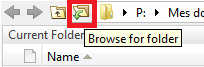
\includegraphics[width=80pt]{../../../img/matlabsimscape/matlab_01} dans le dossier dézippé jusqu'au dossier contenant les fichiers \og .slx \fg\ et \og Simscape \fg,\\
  \begin{center}
  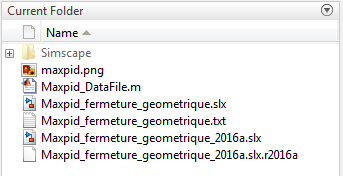
\includegraphics[width=0.3\linewidth]{../../../img/matlabsimscape/matlab_02}
  \end{center}
 \item Faire un clic-droit sur le dossier \og Simscape \fg\ et cliquer sur \og Add to Path \fg,\\
  \begin{center}
  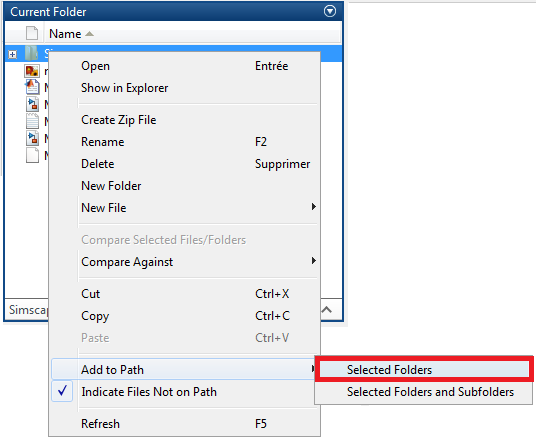
\includegraphics[width=0.4\linewidth]{../../../img/matlabsimscape/matlab_03}
  \end{center}
 \item Double-cliquer sur le fichier correspondant au TP et à la version de Matlab utilisée, il doit avoir une extension en \og slx \fg.\\
  \begin{center}
  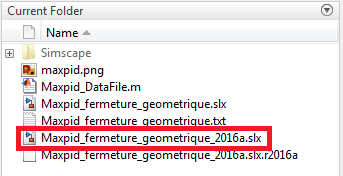
\includegraphics[width=0.4\linewidth]{../../../img/matlabsimscape/matlab_04}
  \end{center}
 \item Afin d'exporter des données, il est nécessaire d'insérer un bloc \textbf{To File} disponible dans la section \textit{Sinks} et de le connecter à la donnée à extraire,
 \item Double-cliquer dessus afin de modifier le paramètre \textit{Save format} en \textbf{Array}. Cela a pour effet de créer un fichier \textit{fichier.mat},
 \item Celui-ci peut être convertit en fichier \textit{fichier.csv} en utilisant les commandes suivantes:
 \texttt{FileData = load('fichier.mat');} \\
 \texttt{csvwrite('fichier.csv', FileData.ans);}
 \end{itemize}	

\label{proceduresimscape}
}

% Boîte d'exercice de maths pures, totalement décontextualisée du SI,
% pour les élèves n'ayant jamais fait de SI. S'utilise en complément
% de \aide (qui, elle, suppose déjà le contexte SI connu).
% Usage: \mathspure{texte}
\newcommand{\mathspure}[1]{%
\medskip\noindent\begin{tikzpicture}
\node[rounded corners=8,inner sep=8pt,fill=success!12,draw=success,line width=0.8pt] (box){%
\begin{minipage}{0.92\linewidth}
\textbf{\textcolor{success}{[M] Maths pures}} \\
\small #1
\end{minipage}
};
\end{tikzpicture}\medskip
}

\newcommand{\aidemecatroisd}{Une ressource permettant la prise en main du logiciel Meca3d est disponible \href{https://atemi.pagesperso-orange.fr/downloads/Meca3d/exemples/v18.0/Sinusmatic_v18.zip}{ici}}

% ------------------------------------------------------------------
% Blocs de différenciation par niveau (aides facultatives / bonus)
% ------------------------------------------------------------------

% Boîte de rappel / aide méthodologique facultative, destinée aux
% élèves qui ont besoin d'un coup de pouce. Usage: \aide{texte}
\newcommand{\aide}[1]{%
\medskip\noindent\begin{tikzpicture}
\node[rounded corners=8,inner sep=8pt,fill=info!12,draw=info,line width=0.8pt] (box){%
\begin{minipage}{0.92\linewidth}
\textbf{\textcolor{info}{[+] Aide / rappel}} \\
\small #1
\end{minipage}
};
\end{tikzpicture}\medskip
}

% Boîte de question bonus / approfondissement, facultative, destinée
% aux élèves les plus à l'aise. Usage: \bonus{texte}
\newcommand{\bonus}[1]{%
\medskip\noindent\begin{tikzpicture}
\node[rounded corners=8,inner sep=8pt,fill=warning!18,draw=warning,line width=0.8pt] (box){%
\begin{minipage}{0.92\linewidth}
\textbf{\textcolor{orange}{[++] Bonus / approfondissement}} \\
\small #1
\end{minipage}
};
\end{tikzpicture}\medskip
}

% Boîte de corrigé associée à une aide ou un bonus (fond neutre gris),
% à utiliser dans la partie \pagestyle{correction}. Usage: \corniveau{texte}
\newcommand{\corniveau}[1]{%
\medskip\noindent\begin{tikzpicture}
\node[rounded corners=8,inner sep=8pt,fill=gris25!15,draw=gris25,line width=0.8pt] (box){%
\begin{minipage}{0.92\linewidth}
\small #1
\end{minipage}
};
\end{tikzpicture}\medskip
}

% Légende à placer en tête de TP pour expliquer la convention [+] / [++]
% aux élèves. Usage: \legendeniveaux
\newcommand{\legendeniveaux}{%
\medskip\noindent\begin{tikzpicture}
\node[rounded corners=8,inner sep=8pt,fill=gris25!10,draw=gris25,line width=0.6pt] (box){%
\begin{minipage}{0.92\linewidth}
\footnotesize
\textbf{\textcolor{success}{[M] Maths pures}} : exercice de maths décontextualisé, pour s'entraîner sur le geste mathématique seul avant de l'appliquer au problème (utile si vous n'avez jamais fait de SI). \\
\textbf{\textcolor{info}{[+] Aide / rappel}} : rappel de cours ou méthode facultative, à utiliser si besoin (les élèves à l'aise peuvent l'ignorer). \\
\textbf{\textcolor{orange}{[++] Bonus}} : question d'approfondissement facultative, à traiter une fois le reste du sujet terminé.
\end{minipage}
};
\end{tikzpicture}\medskip
}





















% En tête et pied de page
\lhead{\nom}
\rhead{
\includegraphics[width=2cm]{../../../img/logo}}
\lfoot{\auteurs}
\cfoot{Page \thepage}

\fancypagestyle{correction}{%
  \fancyhf{}
  \lhead{\colorbox{danger}{\begin{minipage}{0.65\paperwidth} \textcolor{white}{\textbf{Correction}} \end{minipage}} }
  \rhead{
\includegraphics[width=2cm]{../../../img/logo}}
  \lfoot{Renaud Costadoat}
  \rfoot{\colorbox{danger}{\begin{minipage}{0.6\paperwidth} \begin{flushright}\textcolor{white}{\textbf{Correction}}\end{flushright} \end{minipage}} }}

\renewcommand{\footrulewidth}{0.4pt}

\usepackage{eso-pic}
\newcommand{\BackgroundPic}{%
\put(0,0){%
\parbox[b][\paperheight]{\paperwidth}{%
\vfill
\begin{center}
\hspace{0.5cm}\vspace{0.5cm}

\includegraphics[width=\paperwidth,height=\paperheight,%
keepaspectratio]{../../../img/fond3}%
\end{center}
\vfill
}}}

\newcommand{\BackgroundPicdeux}{%
\put(25,-30){%
\parbox[b][\paperheight]{\paperwidth}{%
\vfill
\begin{center}
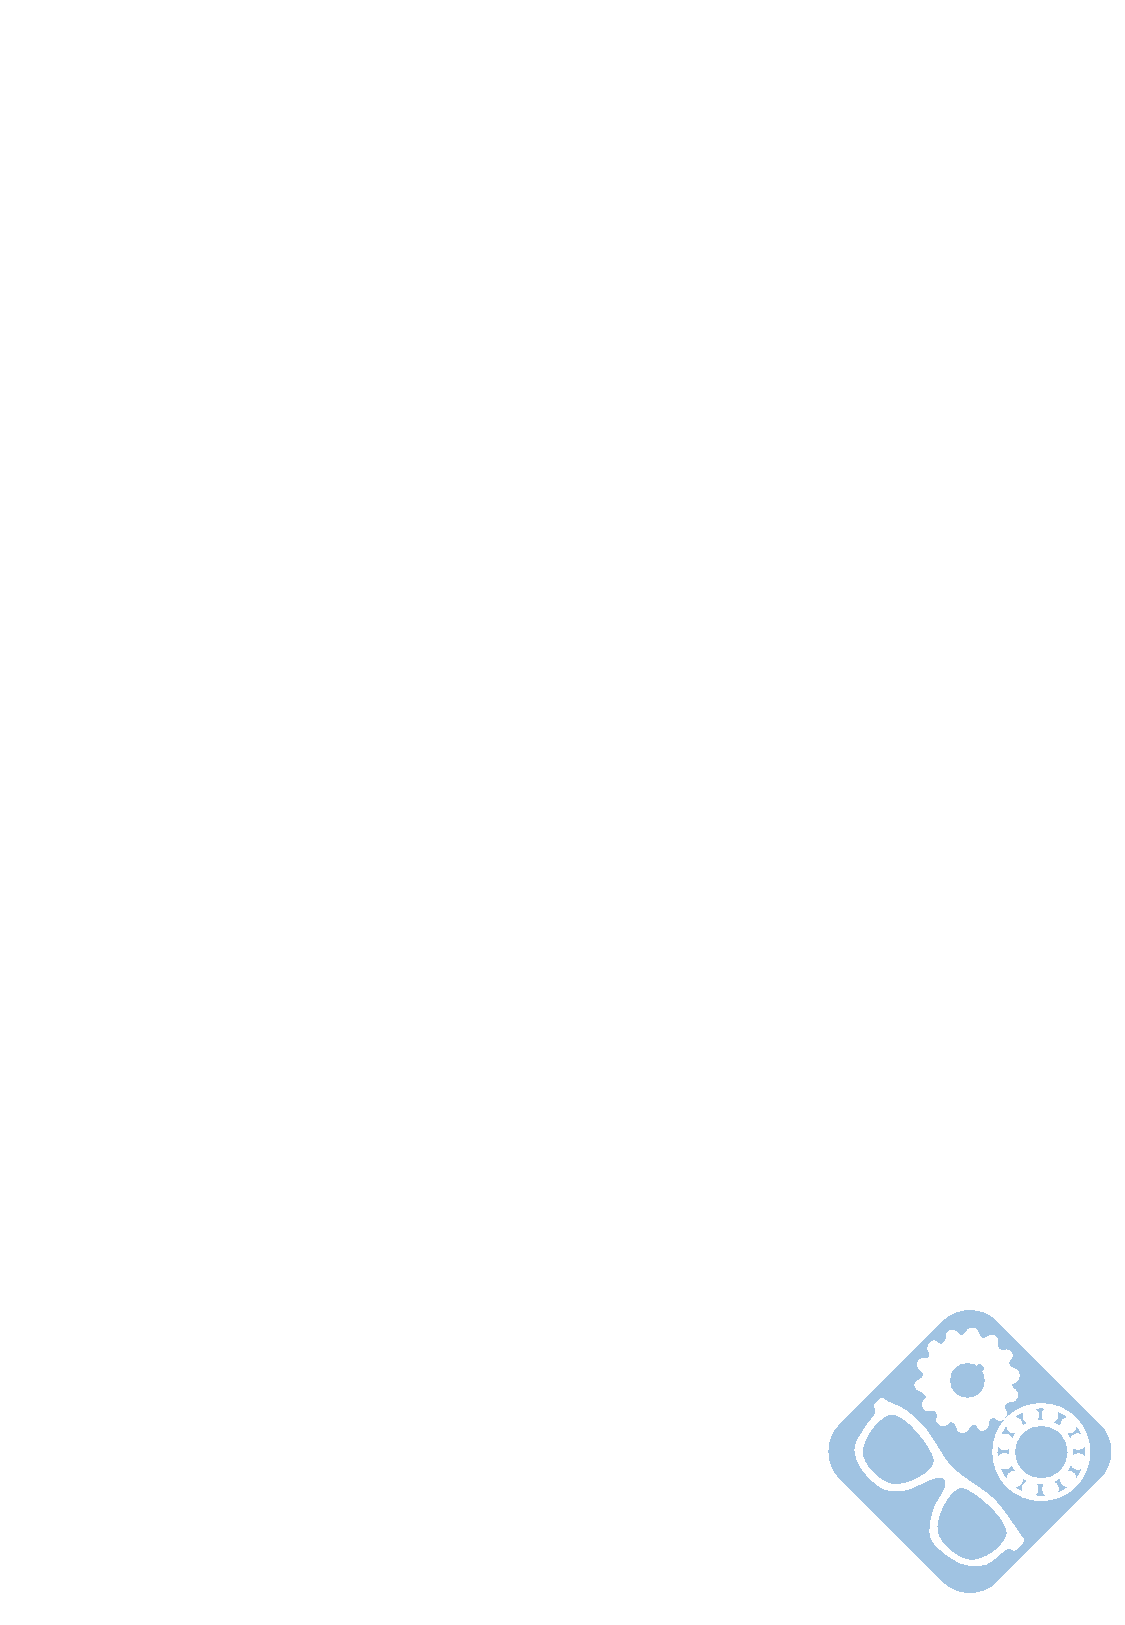
\includegraphics[width=\paperwidth,height=\paperheight,%
keepaspectratio]{../../../img/fond4}%
\end{center}
\vfill
}}}

\newcommand{\activite}[1]{\newpage \cleardoublepage
\renewcommand\arraystretch{2.5}\setcounter{section}{0}\setcounter{subsection}{0}
\ifthenelse{\equal{#1}{1}}{\begin{center}\begin{tabular}{|c|cc p{3cm}|}
\hline
\rowcolor{violt} \supportu & Act & Contenu & Compétences \\\hline
 \multirow{3}{*}{\includegraphics[width=0.2\linewidth]{\supportimageu}} & \begin{LARGE}\textbf{1}\end{LARGE} & \activiteun & \competenceun \\
 & \multicolumn{3}{l|}{Nom: .........................................................................}\\
 & \multicolumn{3}{l|}{Prénom: ....................................................................}\\\hline
\end{tabular}\end{center}}{}
\ifthenelse{\equal{#1}{2}}{\begin{center}\begin{tabular}{|c|cc p{3cm}|}
\hline
\end{tabular}\end{center}}{}}

\begin{document}

\pagestyle{empty}

\vspace*{-3\baselineskip}

\AddToShipoutPicture*{\BackgroundPic}

\ifdef{\auteurdeux}{\begin{tabular}{>{\columncolor{gray!00}}m{.33\linewidth} m{.27\linewidth} >{\columncolor{gray!00}}m{.3\linewidth}}
Séquence \sequence \ - \type \num \ - Îlot \numprint{\ilot} &  \multirow{3}{*}{\hspace{1cm}
\includegraphics[height=1.5cm]{../../../img/logo}} &  \begin{flushright} \multirow{4}{*}{\hspace{1cm}\includegraphics[height=4cm]{"img/qrcode"}}\end{flushright}\\
 \textbf{\institute} \\
 \auteurun\\
 \auteurdeux
\end{tabular}}{\begin{tabular}{>{\columncolor{gray!00}}m{.3\linewidth} m{.3\linewidth} >{\columncolor{gray!00}}m{.3\linewidth}}
Séquence \sequence \ - \type \num \ - Îlot \numprint{\ilot}  &  \multirow{3}{*}{\hspace{1cm}
\includegraphics[height=1.5cm]{../../../img/logo}} &  \begin{flushright} \multirow{4}{*}{\hspace{1cm}\includegraphics[height=4cm]{"img/qrcode"}}\end{flushright}\\
 \textbf{\institute} \\
 \auteurun
\end{tabular}}

\vspace{1cm}

\begin{center}\colorbox{white}{\huge{\nom}}\end{center}

\vspace{2cm}


\begin{center}\colorbox{white!20}{\includegraphics[height=5cm]{/home/renaud/Documents/Renaud/GitHub/django_education/django_education/static/systemes/\imageun}}\end{center}

\vspace{2cm}



\begin{tabular}{p{.15\linewidth} >{\columncolor{white}}p{.8\linewidth}}
    \rowcolor{gray!20}
    Référence & S\sequence \ - \type\num \ - I\numprint{\ilot} \\
    Compétences & \competences \\
 	\rowcolor{gray!20}
    Description & \descrip \\
    Système & \systemes
  \end{tabular}

\newpage

\AddToShipoutPicture{\BackgroundPicdeux}

\pagestyle{fancy}



\prob{Modéliser les caractéristiques d'un moteur à courant continu.} 

\\

\legendeniveaux

\\

\section{Modèle du moteur électrique à courant continu}

\begin{eqnarray}
u_m(t)=L_m.\frac{di(t)}{dt}+R_m.i(t)+e(t) \\
e(t)=K_e.\omega_m(t) \\
J.\frac{d\omega_m(t)}{dt}=C_m(t)-C_r(t) \\
C_m(t)=K_m.i(t)
\end{eqnarray}

Données:
\begin{itemize}
 \item $u_m(t)$: tension aux bornes du moteur ($V$),
 \item $i(t)$: intensité du courant dans le moteur ($A$),
 \item $e(t)$: force électromotrice ($V$),
 \item $\omega_m(t)$: vitesse de rotation du moteur ($rad.s^{-1}$),
 \item $C_m(t)$: couple moteur ($N.m$),
 \item $C_r(t)$: couple résistant ($N.m$),
 \item $L_m$: inductance de la bobine du moteur ($H$),
 \item $R_m$: résistance électrique interne au moteur ($\Omega$),
 \item $K_e$: constante électrique du moteur ($V.rad^{-1}.s$),
 \item $J$: inertie du moteur ($kg.m^2$),
 \item $K_m$: constante de couple du moteur ($N.m.A^{-1}$).
\end{itemize}

~\

En général, on suppose $K_e=K_m$ pour une MCC.

\paragraph{Question 1:} D'après les équations (1) à (4), \textbf{écrire} une équation liant uniquement $u_m(t)$, $\omega_m(t)$ et $C_m(t)$.

\mathspure{Soit les équations $y=3.x+2$ et $z=5.y-1$. Exprimez $z$ uniquement en fonction de $x$ (sans $y$). Méthode : remplacez $y$ par son expression dans la deuxième équation.}

\aide{partez de l'équation (4) pour exprimer $i(t)$ en fonction de $C_m(t)$. Injectez cette expression dans l'équation (2) pour obtenir $e(t)$ en fonction de $C_m(t)$, puis injectez les deux résultats dans l'équation (1). Vous devez obtenir une équation où seuls apparaissent $u_m(t)$, $C_m(t)$ (et ses dérivées) et $\omega_m(t)$.}

\paragraph{Question 2:} Quelles sont les \textbf{hypothèses} à poser afin de mettre cette équation sous la forme $u_m(t)=K.\omega_m(t)$. Est-ce que cela vous paraît raisonnable de prendre ces hypothèses ?

\mathspure{Soit $f(t)=7$ (une fonction constante au cours du temps). Que vaut $\dfrac{df(t)}{dt}$ ? Plus généralement, que vaut la dérivée par rapport au temps d'une grandeur qui ne varie pas au cours du temps ?}

\aide{un système est en \textbf{régime établi} (ou permanent) lorsque toutes ses grandeurs sont constantes au cours du temps. Que valent alors les dérivées première et seconde de $\omega_m(t)$ par rapport au temps ?}

\bonus{en passant en transformée de Laplace (conditions initiales nulles, sans les hypothèses de régime établi), \textbf{écrire} la fonction de transfert $\dfrac{\Omega_m(p)}{U_m(p)}$ du moteur. Quel est l'ordre de ce système ? Que devient cette fonction de transfert lorsque $p\rightarrow 0$ ? Retrouvez-vous le résultat de la question 2 ?}

\paragraph{Question 3:} En supposant que l'on arrive à mesurer le courant qui traverse le moteur, que devient-il alors possible d'\textbf{estimer} ?

\newpage

\section{Mesure des valeurs caractéristiques du moteur} 

\paragraph{Question 4:} \textbf{Déterminer} un protocole afin de mesurer la tension aux bornes du moteur. Donner la liste du matériel utilisé et ses caractéristiques (sensibilité, plage de mesure...).

\paragraph{Question 5:} \textbf{Déterminer} un protocole afin de mesurer la vitesse de rotation du moteur à l'aide du tachymètre. Donner les caractéristiques du matériel (sensibilité, plage de mesure...).

\paragraph{Question 6:} \textbf{Mettre en \oe uvre} ce protocole pour des tensions allant de 0V à 12V. Écrire les valeurs mesurés dans le script python à télécharger 
\href{https://github.com/Costadoat/Sciences-Ingenieur/raw/master/S01\%20\nomsequence/TP01\%20Mod\%C3\%A9lisation\%20lin\%C3\%A9aire/Ilot_01\%20Moteur\%20\%C3\%A0\%20courant\%20continu/01-TP01-I01.py}{ici} 
et l'utiliser afin de tracer la courbe $\omega_m(t)=f(u_m(t))$. Conclure quant à l'allure de ce tracé, quel modèle peut-on appliquer à ce phénomène ?

\mathspure{Une droite passe par les points $(2,4)$ et $(5,13)$. Calculez son coefficient directeur $a$ (pente), défini par $a=\dfrac{y_2-y_1}{x_2-x_1}$. Sachant que l'équation de la droite s'écrit $y=a.x+b$, calculez ensuite $b$ en remplaçant $x$, $y$ et $a$ par leurs valeurs dans l'un des deux points.}

\aide{une fonction affine s'écrit $y=a.x+b$. Sur votre tracé, $a$ correspond à la pente de la droite et $b$ à son ordonnée à l'origine. Comment calculeriez-vous $a$ "à la main" à partir de deux points quelconques $(x_1,y_1)$ et $(x_2,y_2)$ de la courbe ? Faites l'application numérique avec deux points de votre tracé pour vérifier la cohérence avec le résultat donné par le script python.}

\bonus{en reprenant l'expression de la fonction de coût $MSE(\theta)$ donnée en annexe, retrouvez par le calcul (en annulant la dérivée partielle) la formule de l'équation normale $\hat{\Theta}=(X^TX)^{-1}X^Ty$ dans le cas d'un modèle à un seul paramètre $y=\theta_1.x$.}

\paragraph{Question 7:} \textbf{Refaire} la mesure précédente en mesurant aussi le courant qui traverse le moteur.

\paragraph{Question 8:} \textbf{Proposer} et \textbf{mettre en \oe uvre} un protocole permettant de mesurer la résistance interne du moteur. Donner la liste du matériel utilisé et ses caractéristiques (sensibilité, plage de mesure...).

\mathspure{Dans l'équation $y=a.x$, isolez $a$ en fonction de $x$ et $y$ (rappel : on divise les deux membres de l'égalité par la même quantité, ici $x$).}

\aide{la loi d'Ohm $u=R.i$ relie une tension et un courant à travers une résistance. Dans quelles conditions (régime établi ou non) l'équation (1) du modèle se ramène-t-elle à une loi d'Ohm entre $u_m(t)$ et $i(t)$ ?}

\section{Vérification des modèles et analyse des résultats}

\paragraph{Question 9:} À partir des résultats précédents, \textbf{déterminer} le couple résistant $C_r(t)$ pour le moteur libre. \textbf{Proposer} une solution permettant d'augmenter ce couple, \textbf{prédire} le comportement du système.

\mathspure{Sachant que $C=K.i$, calculez $C$ pour $K=0{,}05$ et $i=2{,}3$. N'oubliez pas de préciser l'unité du résultat à partir des unités de $K$ et $i$.}

\aide{d'après la question 3, en régime établi, $C_r(t)=K_e.i(t)$. Il vous suffit donc de reprendre la mesure de $i(t)$ à vide obtenue précédemment et la valeur de $K_e$ déterminée à la question 6 pour faire l'application numérique.}

\subsection{Vérifier expérimentalement un modèle théorique}

\paragraph{Question 10:} \textbf{Mettre en \oe uvre} ce nouveau protocole et \textbf{conclure} quant à la validité de la prédiction de la question 9.

\subsection{Déterminer la valeur de $L_m$}

\paragraph{Question 11:} \textbf{Proposer} sans les mettre en \oe uvre des protocoles permettant de déterminer la valeur de $L_m$.

\section{Synthèse du TP}

\paragraph{Question 12:} \textbf{Conclure} quant au modèle obtenu pour ce moteur à courant continu, \textbf{réaliser} une synthèse de ce TP présentant votre démarche pour répondre à la problématique.

\section{Annexes}

\subsection{Régression linéaire}

A partir d'un ensemble de couples de valeurs $(x_i,y_i)$, le but de la régression linéaire et la prédiction d'un modèle linéaire: \\
\begin{center}
$\hat{y}=\theta_0+\theta_1\cdot x_1+\theta_2\cdot x_2+...+\theta_n\cdot x_n$ \\
$\hat{y}=X \Theta$
\end{center}

Ainsi, il faut trouver l'ensemble des $\theta_i$ qui minimisent l'écart (RMSE Root Mean Square Error ou critère des moindres carrés) entre $y=[y_0, y_1,...,y_n]$ et $\hat{y}$. Pour la suite, on utilisera la MSE car le min de la RMSE est aussi celui de la MSE.

Il existe alors 2 solutions l'équation normale et la descente de gradient.

\paragraph{Équation normale} ~\ \\

Il existe une solution analytique pour trouver la valeur de $\Theta$ qui minimise l'écart.
\begin{center}
$\hat{\Theta}=(X^TX)^{-1}X^Yy$
\end{center}

Fonction python
\begin{lstlisting}
def regression_lineaire_eq_normale(x,y):
    X_b = np.array([[xi] for xi in x])
    theta_best = np.linalg.inv(X_b.T.dot(X_b)).dot(X_b.T).dot(y)
    return theta_best
\end{lstlisting}

\paragraph{Descente de gradient} ~\ \\

La descente de gradient est un algorithme d'optimisation très général, capable de trouver des solutions optimales à un grand nombre de problèmes. 

L'idée générale de la descente de gradient est de corriger petit à petit les paramètres dans le but de minimiser une fonction de coût.

L'algorithme suit la pente de la descente de la fonction MSE vers le bas pour la minimiser.

Dans le cas où il y aurait plusieurs variables il faudrait les normaliser afin que l'impact de leur variation soit identique, ce n'est pas le cas pour notre étude.

La descente de gradient consiste à calculer la dérivée partielle (cf cours de math)
\begin{center}
$\dfrac{\partial}{\partial \theta_j}MSE(\theta)=\dfrac{2}{m}\sum\limits_{i=1}^m (\Theta^T x^{(i)}-y^{(i)})x_j^{(i)}$
\end{center}

On prendra en entrée:
\begin{itemize}
 \item $\eta$: le taux d'apprentissage qui correspond à la taille des pas que l'on effectue dans la descente (plus $\eta$ est grand, plus vite on converge, mais cela peut générer de l'instabilité),
 \item le nombre d'itérations
\end{itemize}

Fonction python
\begin{lstlisting}
def regression_lineaire_descente_gradient(x,y):
    X_b = np.c_[np.ones((len(x), 1)), x]
    eta = 0.1 # taux d'apprentissage (vitesse à laquelle on suit la pente)
    n_iterations = 1000 # tester plusieurs valeurs
    m = 2 # nombre de paramètres
    theta = np.random.randn(2,1)    # initialisation aléatoire de la solution
    for iteration in range(n_iterations):
        gradients = 2/m * X_b.T.dot(X_b.dot(theta) - y)
        theta = theta - eta * gradients
    return theta
\end{lstlisting}

\ifdef{\public}{\end{document}}{}

\clearpage

\newpage

\pagestyle{correction}

\section{Correction}

\paragraph{Question 1:} D'après les équations (1) à (4), \textbf{écrire} une équation liant $u_m(t)$, $\omega_m(t)$ et $C_m(t)$.

$u_m(t)=\frac{L_m}{K_m}.\frac{dC_m(t)}{dt}+\frac{R_m}{K_m}.C_m(t)+K_e.\omega_m(t)$

$u_m(t)=\frac{L_m.J}{K_m}.\frac{d^2\omega_m(t)}{dt^2}+\frac{R_m.J}{K_m}.\frac{d\omega_m(t)}{dt}+K_e.\omega_m(t)$

\corniveau{\textbf{\textcolor{success}{[M] Maths pures :}} en remplaçant $y$ par $3.x+2$ dans $z=5.y-1$, on obtient $z=5.(3.x+2)-1=15.x+10-1=15.x+9$.}

\paragraph{Question 2:} Quelles sont les \textbf{hypothèses} à prendre afin de mettre cette équation sous la forme $u_m(t)=K.\omega_m(t)$.

Il faut se placer à vitesse constante (régime établi) et négliger les frottements, ainsi, $C_r(t)=0$, $\frac{d^2\omega_m(t)}{dt^2}=0$ et $\frac{d\omega_m(t)}{dt}=0$.

Ainsi, $u_m(t)=K_e.\omega_m(t)$

\corniveau{\textbf{\textcolor{success}{[M] Maths pures :}} $\dfrac{df(t)}{dt}=0$. Plus généralement, la dérivée par rapport au temps d'une grandeur constante (qui ne varie pas) est toujours nulle.}

\corniveau{\textbf{\textcolor{orange}{[++] Bonus :}} en transformée de Laplace, $U_m(p)=\left(\dfrac{L_m.J}{K_m}p^2+\dfrac{R_m.J}{K_m}p+K_e\right)\Omega_m(p)$, soit $\dfrac{\Omega_m(p)}{U_m(p)}=\dfrac{K_m}{L_m.J.p^2+R_m.J.p+K_e.K_m}$. C'est un système du second ordre. Lorsque $p\rightarrow 0$, la fonction de transfert tend vers $\dfrac{1}{K_e}$, ce qui redonne bien $u_m(t)=K_e.\omega_m(t)$ en régime permanent, conforme au résultat de la question 2.}

\paragraph{Question 3:} En supposant que l'on arrive à mesurer le courant qui traverse le moteur, que devient-il alors possible de \textbf{mesurer} ?

Il est alors possible de déterminer le couple résistant $C_r(t)$ en régime établi.

Avec $C_m(t)=K_m.i(t)$ et $J.\frac{d\omega_m(t)}{dt}=C_m(t)-C_r(t)=0$ en régime établi, on obtient $C_r(t)=K_m.i(t)=K_e.i(t)$.

\paragraph{Question 6:}

\corniveau{\textbf{\textcolor{success}{[M] Maths pures :}} $a=\dfrac{13-4}{5-2}=\dfrac{9}{3}=3$. En remplaçant dans le premier point : $4=3\times 2+b$, soit $b=4-6=-2$. La droite a donc pour équation $y=3.x-2$.}

\corniveau{\textbf{\textcolor{orange}{[++] Bonus :}} pour un modèle à un seul paramètre $\hat{y}=\theta_1.x$, $MSE(\theta_1)=\dfrac{1}{m}\sum\limits_{i=1}^m(\theta_1.x^{(i)}-y^{(i)})^2$. En annulant sa dérivée : $\dfrac{d}{d\theta_1}MSE(\theta_1)=\dfrac{2}{m}\sum\limits_{i=1}^m x^{(i)}(\theta_1.x^{(i)}-y^{(i)})=0$, soit $\theta_1\sum (x^{(i)})^2=\sum x^{(i)}y^{(i)}$, donc $\theta_1=\dfrac{\sum x^{(i)}y^{(i)}}{\sum (x^{(i)})^2}$. On retrouve bien la forme matricielle $\hat{\Theta}=(X^TX)^{-1}X^Ty$ dans ce cas particulier à une dimension, où $X^TX=\sum(x^{(i)})^2$ (un scalaire) et $X^Ty=\sum x^{(i)}y^{(i)}$.}

\paragraph{Question 8:}

\corniveau{\textbf{\textcolor{success}{[M] Maths pures :}} en divisant les deux membres de $y=a.x$ par $x$, on obtient $a=\dfrac{y}{x}$. Appliqué à la loi d'Ohm $u=R.i$, cela donne $R=\dfrac{u}{i}$, valable en régime établi (continu) puisque l'équation (1) se réduit alors à $u_m(t)=R_m.i(t)+K_e.\omega_m(t)$ à vitesse nulle (moteur bloqué), soit $u_m(t)=R_m.i(t)$.}

\paragraph{Question 9:}

\corniveau{\textbf{\textcolor{success}{[M] Maths pures :}} $C=0{,}05\times 2{,}3=0{,}115\ N.m$.}

\end{document}
